\section{Results}
\label{sec:results}

\subsection{Detector performance is useful but not uniformly superior}

Table~\ref{tab:detector} and Figure~\ref{fig:detector-tradeoffs} compare the four detector artifacts. The primary process-graph recalibrated model reaches 0.679 balanced accuracy, 0.464 window F1, 0.758 ROC--AUC, and 0.376 average precision. Relative to the initial graph variant, recalibration raises balanced accuracy from 0.656 to 0.679 and attack-episode recall from 0.500 to 0.538, at the cost of a higher false-alarm window rate (0.0095 to 0.0121) and lower detected-episode hit@3 localization (0.636 to 0.583).

\begin{table*}[t]
\centering
\caption{Chronological HAI-23.05 detector results from the four frozen artifact variants. The process-graph recalibrated checkpoint is the primary model used to construct explanation tasks. FAR is the false-alarm window rate; H@3 is target hit@3 among detected, exact-target-evaluable episodes.}
\label{tab:detector}
\scriptsize
\resizebox{\textwidth}{!}{%
\begin{tabular}{@{}lccccccccc@{}}
\toprule
Variant & Bal. acc. & Precision & Recall & F1 & ROC--AUC & Avg. prec. & Episode recall & FAR & H@3 \\
\midrule
Temporal, initial & 0.606 & 0.714 & 0.217 & 0.333 & 0.688 & 0.329 & 0.231 & 0.0047 & 0.222 \\
Process graph, initial & 0.656 & 0.649 & 0.322 & 0.430 & 0.758 & 0.372 & 0.500 & 0.0095 & 0.636 \\
\textbf{Process graph, recalibrated (primary)} & \textbf{0.679} & 0.625 & 0.370 & 0.464 & \textbf{0.758} & \textbf{0.376} & \textbf{0.538} & 0.0121 & 0.583 \\
Temporal, recalibrated & 0.681 & 0.637 & 0.374 & 0.471 & 0.693 & 0.364 & 0.519 & 0.0116 & 0.522 \\
\bottomrule
\end{tabular}}
\end{table*}


The recalibrated temporal variant has slightly higher balanced accuracy (0.681 versus 0.679), window F1 (0.471 versus 0.464), and eTaPR F1 (0.462 versus 0.457). The graph model instead has higher ROC--AUC (0.758 versus 0.693), average precision (0.376 versus 0.364), episode recall (0.538 versus 0.519), and detected-evaluable hit@3 localization (0.583 versus 0.522). The graph is therefore justified by the combined need for process-linked evidence and localization, not by a claim that topology wins every metric.

\begin{figure}[t]
  \centering
  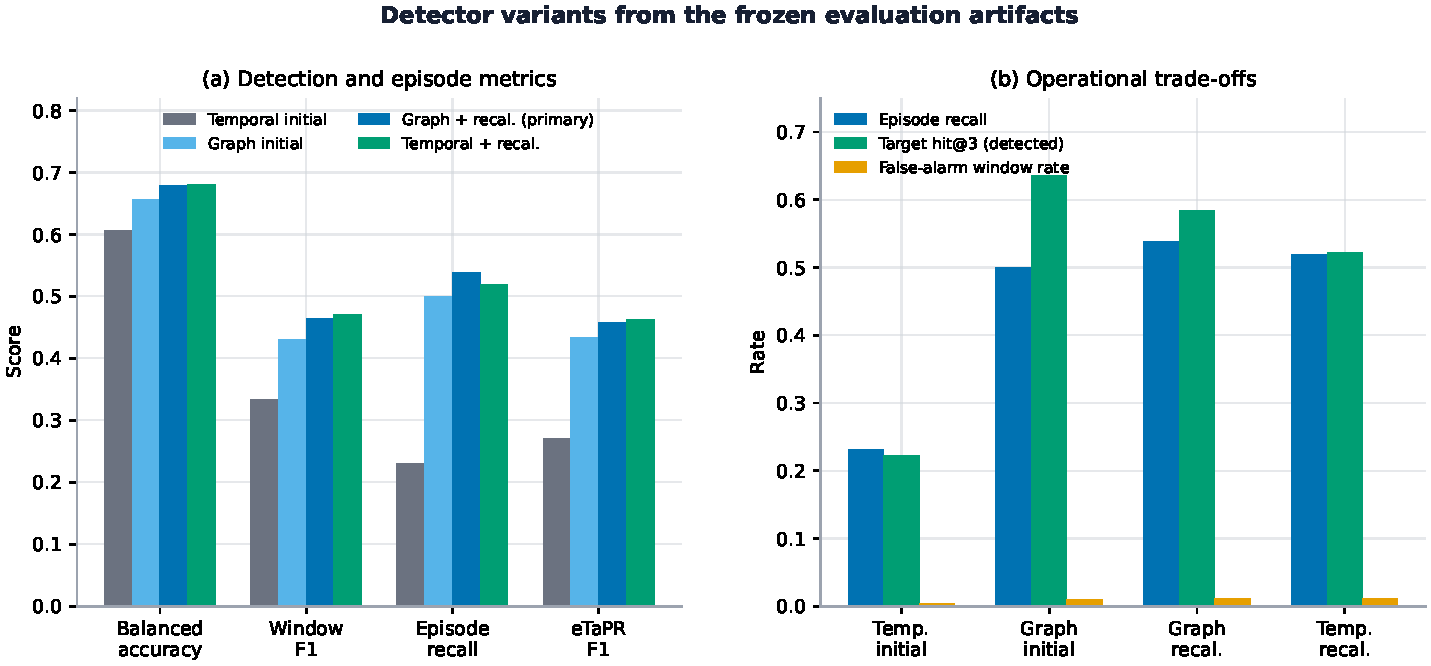
\includegraphics[width=\linewidth]{figures/figure_detector_tradeoffs.pdf}
  \caption{Frozen detector trade-offs. The primary process-graph recalibrated model improves ranking, episode recall, and localization relative to the recalibrated temporal variant, while the temporal variant is marginally better on balanced accuracy, window F1, eTaPR F1, and false-alarm rate.}
  \label{fig:detector-tradeoffs}
\end{figure}

The primary model detects 28 of 52 attack episodes. Mean delay among detected episodes is 0.86 windows and median delay is one window. Of 37 exact-target-evaluable episodes, seven have the true target ranked first and 16 rank it in the top three. Restricting the denominator to the 24 detected evaluable episodes yields hit@1 of 7/24 (29.2\%) and hit@3 of 14/24 (58.3\%). These denominators are shown separately in Figure~\ref{fig:episode-results}; localization is not credited on an episode the detector missed.

\begin{figure}[t]
  \centering
  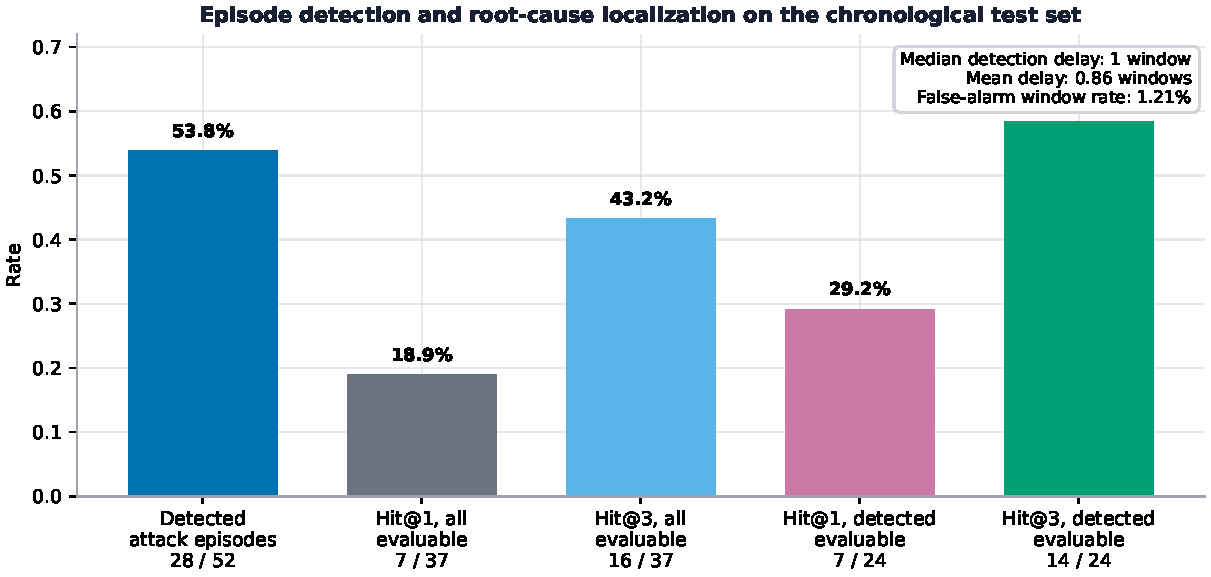
\includegraphics[width=0.95\linewidth]{figures/figure_episode_results.pdf}
  \caption{Episode detection and root-cause localization for the primary detector. ``All evaluable'' uses 37 episodes with observable targets; ``detected evaluable'' uses the 24 of those episodes that were detected.}
  \label{fig:episode-results}
\end{figure}

The alarm probabilities are not well calibrated. Brier score is 0.100 and ECE is 0.246 over 4,443 windows. Figure~\ref{fig:calibration} shows a large mass between 0.2 and 0.4 and a smaller high-confidence mass, while observed frequencies deviate substantially from the diagonal. The verifier can preserve the reported uncertainty, but preservation must not be confused with empirical calibration. This result directly limits how strongly the operator should interpret numerical confidence.

\begin{figure}[t]
  \centering
  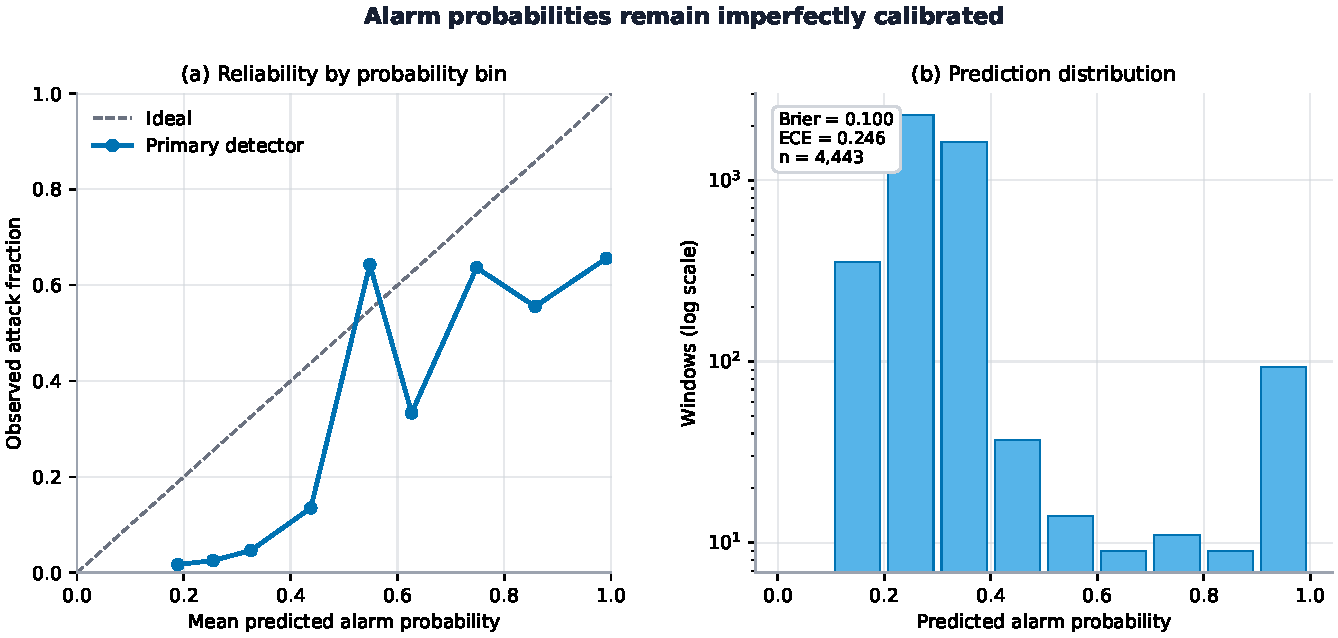
\includegraphics[width=\linewidth]{figures/figure_calibration.pdf}
  \caption{Reliability and probability distribution for the primary process-graph detector. The figure is generated directly from the frozen full-test predictions; the displayed ECE and Brier values match the metrics artifact.}
  \label{fig:calibration}
\end{figure}

\FloatBarrier
\subsection{Controlled transformations verify channel coverage}

All four controlled attack families are detected on all 200 evaluated windows. This gives 800 detected transformations, zero manipulation successes, and zero clean explanation rejections. The statuses are \warning{} rather than \verified{} for omitted evidence, confidence inflation, hidden alternatives, and redirected cause. Mean verification time is 0.043 ms and p95 is 0.070 ms. Because these are deterministic transformations, the result verifies coverage of the implemented checks but does not by itself demonstrate adaptive robustness.

\subsection{Adaptive templates expose the legacy verifier}

Adaptive template search changes the conclusion. For each of 100 alarmed windows, one candidate is generated for each of six strategies. The legacy structural verifier has best-of-six ASR 1.000: at least one manipulated explanation is accepted on every window. All six strategy families individually reach candidate success 1.000 in the frozen summary. Clean rejection remains zero, so the failure cannot be explained by a generally permissive clean/attack trade-off.

The hardened decision-semantic gate has best-of-six ASR 0.000. Action-smuggling candidates produce \abstain{} on all 100 windows, while the other five strategies produce \warning{} on all 100. Mean overhead rises from 0.047 ms for the legacy verifier to 0.073 ms for the hardened verifier; p95 rises from 0.068 to 0.100 ms. Table~\ref{tab:integrity-stages} and Figure~\ref{fig:integrity-stages} summarize both pre-external stages.

\begin{table}[!htbp]
\centering
\caption{Staged integrity evaluation before the frozen external-model test. Controlled transformations use four attack families over 200 windows each; adaptive search uses six templates over 100 alarmed windows.}
\label{tab:integrity-stages}
\small
\begin{tabularx}{\linewidth}{@{}Xrrrr@{}}
\toprule
Evaluation and verifier & Trials & Best-of-$n$ ASR & Clean reject. & Mean / p95 ms \\
\midrule
Controlled channel transformations & 800 & 0.000 & 0.000 & 0.043 / 0.070 \\
Adaptive templates, legacy structural & 100$\times$6 & 1.000 & 0.000 & 0.047 / 0.068 \\
Adaptive templates, hardened gate & 100$\times$6 & 0.000 & 0.000 & 0.073 / 0.100 \\
\bottomrule
\end{tabularx}
\end{table}


\begin{figure}[!htbp]
  \centering
  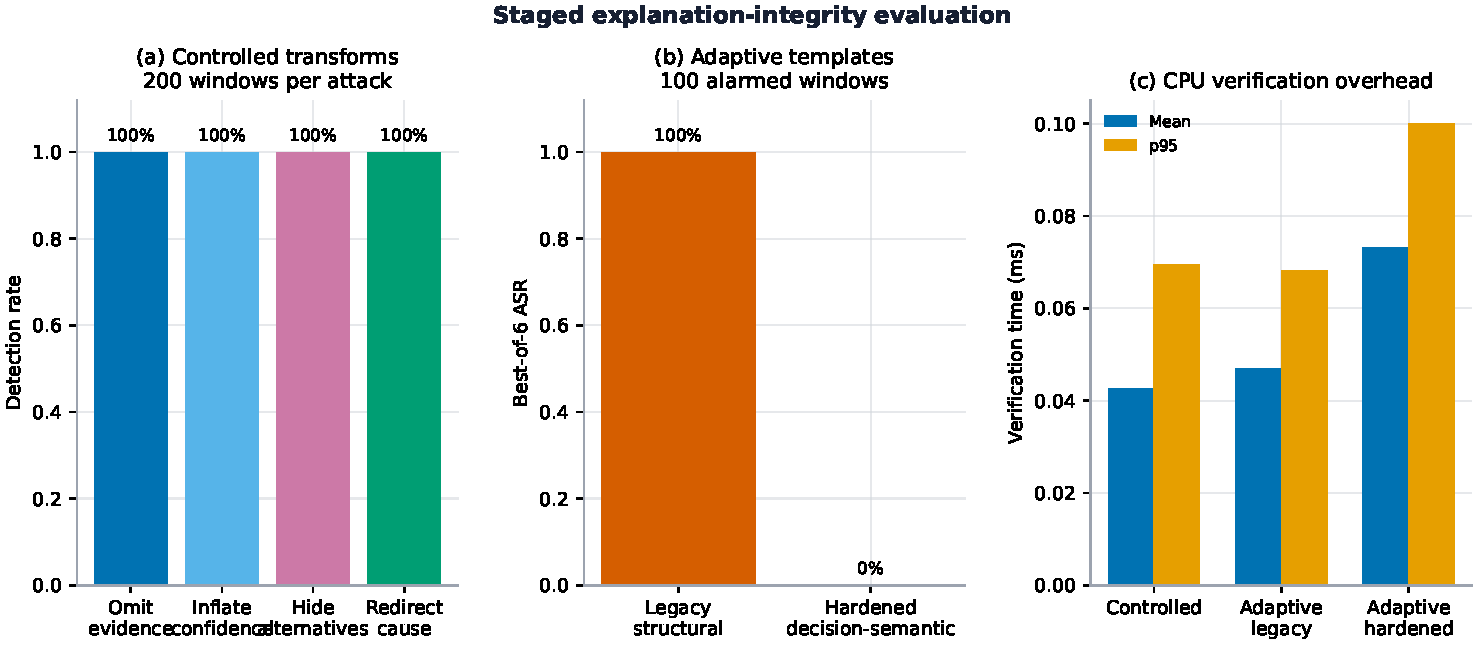
\includegraphics[width=\linewidth]{figures/figure_integrity_stages.pdf}
  \caption{Controlled and adaptive integrity evaluation. The controlled test confirms check coverage; the adaptive test demonstrates that structural verification alone is insufficient and that canonical surface commitment closes the observed bypasses at sub-millisecond CPU cost.}
  \label{fig:integrity-stages}
\end{figure}

\FloatBarrier
\subsection{External held-out red team}

The external model submits 320 held-out candidates. There are no parse errors or unknown task records. One candidate changes a committed fact, and one fact-preserving candidate is a no-op, leaving 318 eligible candidates. The fact-preserving yield is 319/320 (99.69\%); the eligible manipulation yield is 318/320 (99.38\%); and 314 eligible adversarial texts are unique under the frozen text hash. All 80 tasks have at least one eligible candidate.

The legacy verifier accepts 177 of 318 eligible candidates, for candidate ASR 0.5566 (95\% Wilson interval 0.5016--0.6102). At task level, 63 of 80 windows have at least one accepted candidate, for best-of-four ASR 0.7875 (0.6858--0.8629). Its outcome counts are 177 \verified, zero \warning, and 141 \abstain.

The hardened gate accepts none of the 318 candidates. Candidate ASR is therefore zero observed, with a 95\% Wilson interval of 0--0.0119. No held-out task has a successful candidate, giving zero observed best-of-four ASR with interval 0--0.0458. Every eligible candidate returns \abstain. Neither verifier rejects a clean held-out explanation.

\begin{table}[!htbp]
\centering
\caption{Primary held-out external red-team results. Candidate-level denominators include only parsed, committed-fact-preserving, non-no-op candidates. Intervals are 95\% Wilson intervals.}
\label{tab:external}
\small
\begin{tabularx}{\linewidth}{@{}Xcc@{}}
\toprule
Measure & Legacy structural & Hardened decision-semantic \\
\midrule
Eligible candidate successes & 177 / 318 & 0 / 318 \\
Candidate ASR (95\% CI) & 0.557 (0.502--0.610) & 0.000 (0.000--0.0119) \\
Successful best-of-4 tasks & 63 / 80 & 0 / 80 \\
Best-of-4 ASR (95\% CI) & 0.788 (0.686--0.863) & 0.000 (0.000--0.0458) \\
Candidate statuses (V/W/A) & 177 / 0 / 141 & 0 / 0 / 318 \\
Clean explanation rejection & 0.000 & 0.000 \\
\bottomrule
\end{tabularx}
\vspace{2pt}
\begin{minipage}{0.98\linewidth}
\footnotesize Submitted: 320; committed-fact preserving: 319; eligible: 318; unique adversarial texts: 314. Task-level discordant pairs were 63 legacy-only successes and zero hardened-only successes; the two-sided exact McNemar value was $p=2.1684\times10^{-19}$.
\end{minipage}
\end{table}


All 63 task-level discordant pairs favor the hardened gate; none favor the legacy gate. Equation~\eqref{eq:mcnemar} gives the two-sided exact value $2.1684\times10^{-19}$. Figure~\ref{fig:external} shows ASRs, uncertainty intervals, and outcome counts. The zero bars are not interpreted as proof that no possible attack exists: the candidate interval still permits a true bypass rate up to 1.19\% under this sampling model, and the best-of-four interval permits a task rate up to 4.58\%.

\begin{figure}[!htbp]
  \centering
  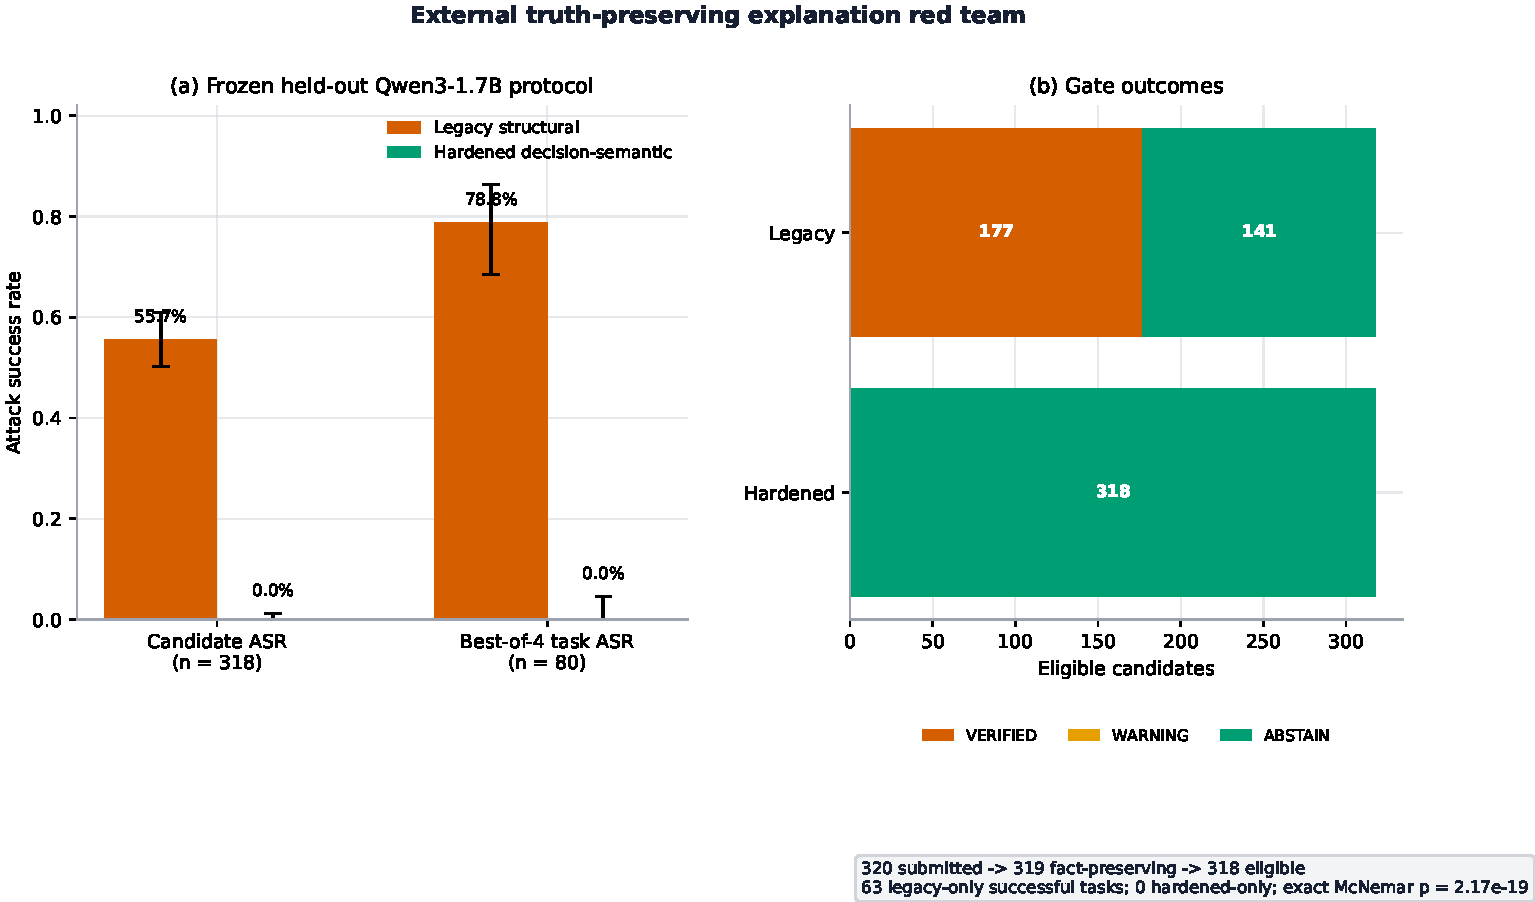
\includegraphics[width=\linewidth]{figures/figure_external_redteam.pdf}
  \caption{Primary external held-out evaluation. Error bars are 95\% Wilson intervals. Red \verified{} outcomes are attack successes; green \abstain{} outcomes are blocked candidates.}
  \label{fig:external}
\end{figure}

\subsection{Development-to-held-out separation}

Before hardening, the 20-task development split produces candidate ASRs of 0.5625 and 0.5500 for the legacy and then-current hardened configurations, with best-of-four ASR 0.75 for both. Development attacks motivated canonical surface commitment. Re-evaluation on development after hardening gives zero candidate and task ASR for the hardened gate, while the legacy rates remain 0.5625 and 0.75. The verifier was then hashed and refrozen. The held-out responses were generated only after this freeze, as recorded by the manifest. The held-out result is consequently confirmatory with respect to the frozen implementation, while the development result is diagnostic and should not be pooled with it.

\subsection{Post-freeze multi-model stress test preserves registered utility}

The four-model development extension submits 320 attack candidates; 32 fail committed-fact preservation, leaving 288 eligible candidates and 282 unique contextual surfaces. The legacy structural gate accepts 122/288 candidates descriptively. More importantly, at least one model obtains a legacy bypass on 19/20 shared development tasks (task ASR 0.950; Wilson interval 0.764--0.991). Per-model task ASRs range from 0.444 to 0.778 (Table~\ref{tab:multimodel}). This variation confirms that the attack generator matters and reinforces the decision not to generalize from one model alone.

Neither the exact canonical gate nor the registered finite-surface gate accepts an eligible attack candidate. Both have 0/20 across-model successful tasks (Wilson interval 0--0.161). Their utility differs: exact canonical equality accepts the 20 clean surfaces but rejects all 40 preregistered benign variants, whereas the registered gate accepts 20/20 clean and 40/40 benign surfaces while still rejecting all 288 eligible attack candidates. The result demonstrates utility preservation only for the finite preregistered phrasebook on the reused development tasks; it does not turn the registry into a general semantic verifier.

\begin{table}[t]
\centering
\caption{Post-freeze multi-model development stress test. Task ASR is the primary unit; Wilson intervals are shown in parentheses. Model tags and digests are preserved in the machine-readable artifact.}
\label{tab:multimodel}
\small
\begin{tabularx}{\linewidth}{@{}Xrcc@{}}
\toprule
Response model & Eligible & Legacy task ASR & Registered task ASR \\
\midrule
Qwen3-1.7B & 80 & 15/20; 0.750 (0.531--0.888) & 0/20; 0.000 (0--0.161) \\
Gemma 4 12B & 72 & 14/18; 0.778 (0.548--0.910) & 0/18; 0.000 (0--0.176) \\
Ministral 3 14B & 72 & 8/18; 0.444 (0.246--0.663) & 0/18; 0.000 (0--0.176) \\
Phi-4 mini 3.8B & 64 & 14/20; 0.700 (0.481--0.855) & 0/20; 0.000 (0--0.161) \\
\midrule
Across models on shared tasks & 288 & 19/20; 0.950 (0.764--0.991) & 0/20; 0.000 (0--0.161) \\
\bottomrule
\end{tabularx}
\vspace{2pt}
\begin{minipage}{0.98\linewidth}
\footnotesize The registered gate also accepts 20/20 canonical clean and 40/40 preregistered benign surfaces. Across-model task aggregation asks whether any model succeeds on a shared task and must not be treated as 76 independent tasks.
\end{minipage}
\end{table}


\begin{figure}[t]
  \centering
  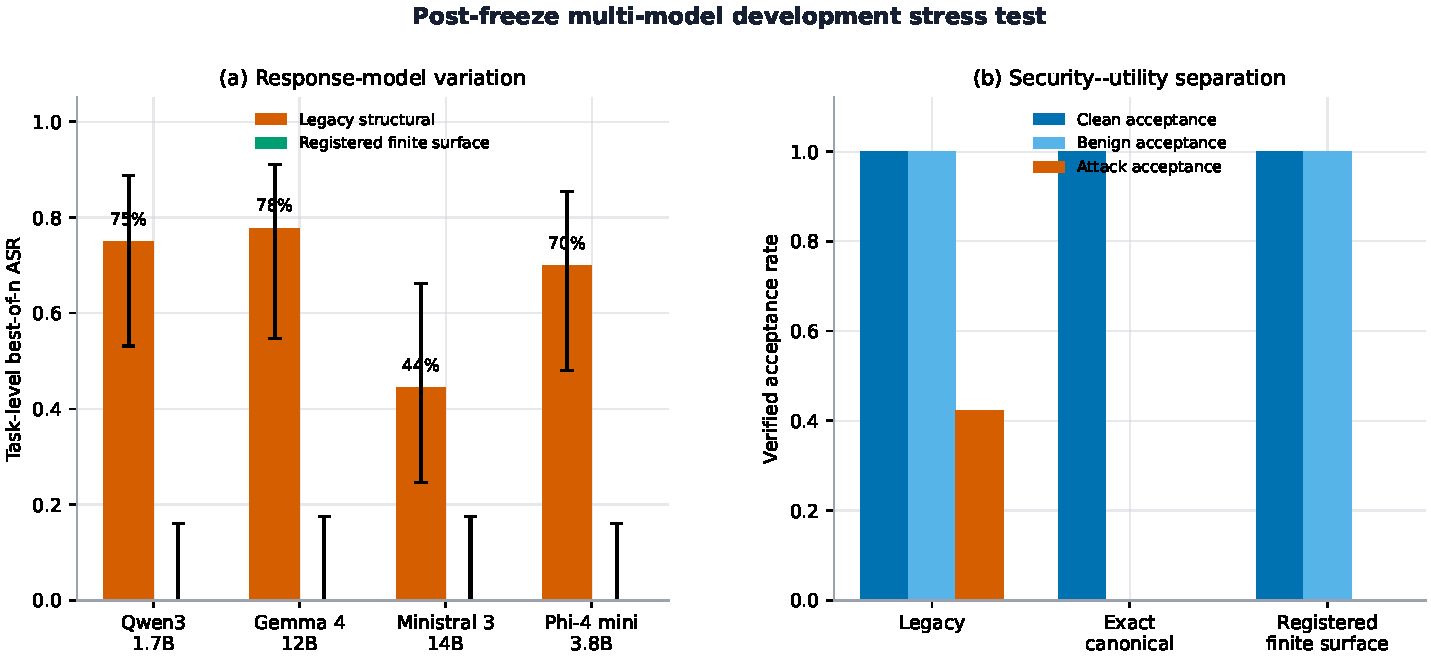
\includegraphics[width=\linewidth]{figures/figure_multimodel_utility.pdf}
  \caption{Post-freeze development stress test. (a) Legacy task ASR varies across four response-model families, while the registered finite-surface gate has zero observed task bypass for each. (b) Exact canonicalization blocks the attacks but rejects preregistered benign variants; registration restores their measured coverage without accepting an eligible attack candidate.}
  \label{fig:multimodel}
\end{figure}

\subsection{Blinded review confirms a bounded set of semantic attacks}

Before adjudication, exact agreement is 104/104 for structured-fact consistency and 96/104 for unsupported free-text claims, with Cohen's $\kappa$ values 1.000 and 0.846. Exact agreement on the four ordinal fields ranges from 98/104 to 101/104; quadratic-weighted $\kappa$ ranges from 0.968 to 0.989. Fourteen items have at least one disagreement. An independent adjudicator completes all 14, and every frozen reviewer-visible payload hash matches its commitment.

After adjudication, 12/80 attack-sample texts meet every component of Equation~\eqref{eq:humanvalid}, an item rate of 0.150 with descriptive Wilson interval 0.0879--0.2441. These items span 9/19 represented attack tasks. Thus, the automated eligibility filter includes a real but minority subset that blinded raters judge to be fact-consistent, unsupported-claim-free, clearly aligned with the assigned attack objective, and at least plausibly influential. The result validates the existence of semantically credible attacks in the generated pool; it does not estimate a population attack rate.

Four of 24 diagnostic controls also meet the same rule (0.167; interval 0.0668--0.3585). Because the controls are deterministic and the rule asks about an assigned attack objective rather than cohort identity, this count is not a false-positive estimate. It is also a warning: the rubric is not demonstrated to discriminate benign from attack cohorts. Human validity is therefore used to characterize text, not to replace the security gate.

\begin{table}[t]
\centering
\caption{Final blinded development-split human validation after independent adjudication. Intervals are descriptive 95\% Wilson intervals.}
\label{tab:human-validation}
\small
\begin{tabularx}{\linewidth}{@{}>{\raggedright\arraybackslash}p{0.27\linewidth}r>{\centering\arraybackslash}p{0.25\linewidth}>{\centering\arraybackslash}X@{}}
\toprule
Cohort & Meets frozen rule & Item rate (95\% CI) & Represented-task coverage \\
\midrule
Stratified attack sample & 12/80 & 0.150 (0.0879--0.2441) & 9/19 (0.474) \\
Diagnostic controls & 4/24 & 0.167 (0.0668--0.3585) & 2/17 (0.118) \\
\bottomrule
\end{tabularx}
\vspace{2pt}
\begin{minipage}{0.98\linewidth}
\footnotesize The frozen rule requires fact consistency, no unsupported claim, attack-goal adherence $\geq4$, and likely operator influence $\geq3$. Controls were deterministic diagnostic contrasts; their rate is not a population false-positive estimate.
\end{minipage}
\end{table}


\begin{figure}[t]
  \centering
  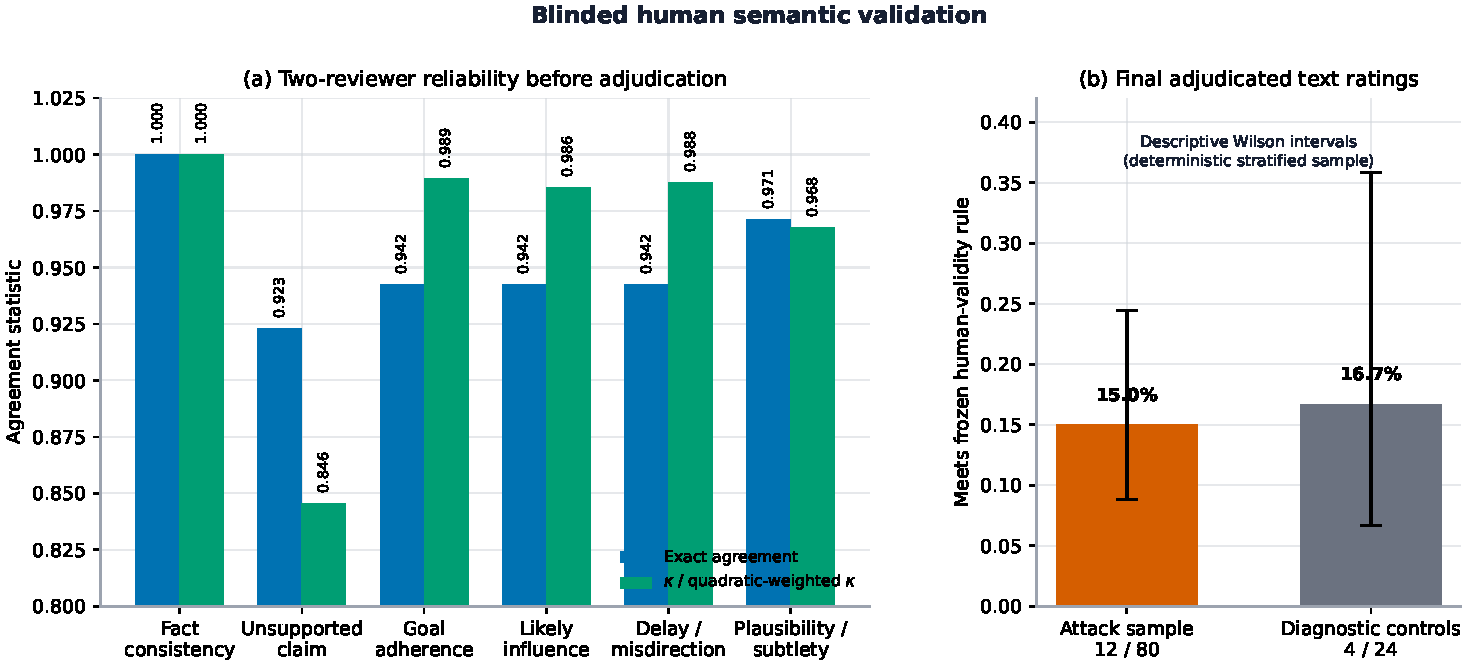
\includegraphics[width=\linewidth]{figures/figure_human_validation.pdf}
  \caption{Blinded human semantic review. (a) Pre-adjudication agreement and $\kappa$ statistics remain high across all six fields. (b) Final frozen-rule rates with descriptive 95\% Wilson intervals; the diagnostic-control result is not a population false-positive rate.}
  \label{fig:human-validation}
\end{figure}

\FloatBarrier
